\section{The Real Line and Coordinate Plane. Pythagoras}
\begin{introduction}
  \item The real line
  \item Inequalities
  \item Absolute values
  \item Intervals
  \item The coordinate plane
  \item The distance formula
  \item The midpoint formula
  \item Note on Pythagoras
\end{introduction}
\begin{questions}
  \item Among the words ``integer'', ``rational'', and ``irrational'', state the ones that apply to
  \begin{tasks}(4)
    \task \(-\frac{2}{3}\);
    \task \(0\);
    \task \(\frac{45}{9}\);
    \task \(0.75\);
    \task \(-\sqrt{49}\);
    \task \(\frac{1}{\pi}\);
    \task \(9.000...\);
    \task \(3^{1/2}\);
    \task \(-\frac{20}{7}\);
    \task \(\frac{94}{7}\).
  \end{tasks}
  \begin{note}
    \begin{itemize}
      \item \(\frac{45}{9} = 5\)
      \item \(-\sqrt{49} = -7\)
      \item \(9.000... = 9\)
    \end{itemize}
  \end{note}
  \begin{solution}
    \begin{itemize}
      \item integer: \(0\), \(\frac{45}{9}\), \(-\sqrt{49}\), \(9.000...\);
      \item rational: \(-\frac{2}{3}\), \(0.75\), \(-\frac{20}{7}\), \(\frac{94}{7}\);
      \item irrational: \(\frac{1}{\pi}\), \(3^{1/2}\).
    \end{itemize}
  \end{solution}
  \item Every integer is either even or odd. The even integers are those that are divisible by $2$, so $n$ is even if and only if it has the form $n=2k$ for some integer $k$. The odd integers are those that have the form $n=2k + 1$ for some integer $k$.
  \begin{tasks}
    \task If $n$ is even, prove that $n^2$ is also even.
    \task If $n$ is odd, prove that $n^2$ is also odd.
  \end{tasks}
  \begin{proof}
    \begin{tasks}
      \task Let $n$ be an even integer. By definition, there exist an integer $k$ such that $n=2k$.

      Consider $n^2$:

      $n^2=(2k)^2=4k^2=2(2k^2)$

      Since $2k^2$ is an integer, $n^2$ can be expressed in the form of $2m$ for integer $m=2k^2$, which implies that $n^2$ is even.

      Therefore, if $n$ is even, then $n^2$ is also even.
      \task Let $n$ be an odd integer. By definition, there exist an integer $k$ such that $n=2k+1$.

      Consider $n^2$:

      $n^2=(2k+1)^2 = 4k^2+4k+1=2(2k^2+2k) + 1$

      Since $2k^2+2k$ is an integer, $n^2$ can be expressed in the form of $n = 2m+1$ for integer $m=2k^2+2k$, which implies that $n^2$ is odd.

      Therefore, if $n$ is odd, then $n^2$ is also odd.
    \end{tasks}
  \end{proof}
  In Problems 3-12, rewrite the given expression without using the absolute value symbol.
  \begin{solution}
    \item $ \left| 7 - 18 \right| = 11 $.
    \item $ \left| 7 \right| - \left| - 18 \right| = -11 $.
    \item $ \left| \pi - 3\right| = \pi - 3 $.
    \item $ \left| 3 - \pi \right| = \pi - 3 $.
    \item $ \left| x - 5 \right| = 5 - x $ if $ x < 5 $.
    \item $ \left| x - 5 \right| = x - 5 $ if $ x > 5 $.
    \item $ \left| x^2 + 10 \right| = x^2 + 10$.
    \item $ \left| -11 \right| - \left| -10 \right| = 1 $.
    \item $ \left| 1 - 3x^2 \right| = 3x^2 - 1 $ if $ x \geq 1 $.
    \item $ \left| \sqrt{10} - 10 \right| = 10 - \sqrt{10} $.
  \end{solution}
  \item Solve the following inequalities:
  \begin{tasks}(3)
    \task $ x(x - 1) > 0 $;
    \task $ (x - 1)(x + 2) < 0 $;
    \task $ x^2 + 4x - 21 > 0 $;
    \task $ 2x^2 + x < 3 $;
    \task $ 4x^2 + 10x - 6 < 0 $;
    \task $ x^2 + 2x + 4 > 0 $;
  \end{tasks}
  \begin{note}
    \begin{multicols}{2}
      \begin{tikzpicture}
        % Define the center and axis lengths of the hyperbola
        \def\a{2}

        % Draw the x axis
        \draw[->] (-3,0) -- (3,0) node[right] {$x$};

        % Draw the parabola
        \draw[domain=-2:2,smooth,variable=\x,blue] plot ({\x},{(\x)^2 - \a});

        % Draw the vertices
        \filldraw[blue] ({sqrt(\a)},0) circle (1pt) node[below right] {root};
        \filldraw[blue] ({-sqrt(\a)},0) circle (1pt) node[below left] {root};

        % Write text at a specific position
        \node[right] at (2,1) {$+$};
        \node[left] at (-2,1) {$+$};
        \node[above] at (0,-1) {$-$};

      \end{tikzpicture}
      \columnbreak

      Quick tips for quadratic functions:
      \begin{enumerate}
        \item Draw the $x$-axis and plot the function.
        \item Mark where it crosses the $x$-axis.
        \item For $x > 0$, it's above the axis. For $x < 0$, it's below.
        \item If the quadratic term's negative, flip the graph!
      \end{enumerate}
    \end{multicols}
  \end{note}
  \begin{solution}
    \begin{tasks}(2)
      \task $ x(x - 1) > 0 $;
      {
        \begin{note}
        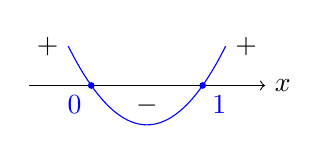
\begin{tikzpicture}
          \def\a{0.5}
          \draw[->] (-1.5,0) -- (1.5,0) node[right] {$x$};
          \draw[domain=-1:1,smooth,variable=\x,blue] plot ({\x},{(\x)^2 - \a});
          \filldraw[blue] ({-sqrt(\a)},0) circle (1pt) node[below left] {$0$};
          \filldraw[blue] ({sqrt(\a)},0) circle (1pt) node[below right] {$1$};
          \node[right] at (1,0.5) {$+$};
          \node[left] at (-1,0.5) {$+$};
          \node[above] at (0,-0.5) {$-$};
        \end{tikzpicture}
      \end{note}
      $x<0$ and $x>1$
      }
      \task $ (x - 1)(x + 2) < 0 $;
      {
        \begin{note}
          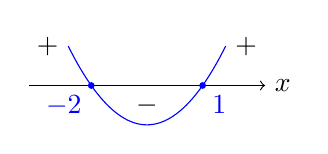
\begin{tikzpicture}
            \def\a{0.5}
            \draw[->] (-1.5,0) -- (1.5,0) node[right] {$x$};
            \draw[domain=-1:1,smooth,variable=\x,blue] plot ({\x},{(\x)^2 - \a});
            \filldraw[blue] ({-sqrt(\a)},0) circle (1pt) node[below left] {$-2$};
            \filldraw[blue] ({sqrt(\a)},0) circle (1pt) node[below right] {$1$};
            \node[right] at (1,0.5) {$+$};
            \node[left] at (-1,0.5) {$+$};
            \node[above] at (0,-0.5) {$-$};
          \end{tikzpicture}
        \end{note}
        $-2<x<1$
      }
      \task $ x^2 + 4x - 21 > 0 $;
      {
        \begin{note}
          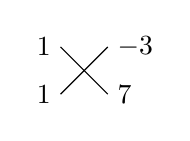
\begin{tikzpicture}
            \def\a{0.3}
            \draw[-] (-\a,\a) node[left] {$1$} -- (\a,-\a) node[right] {$7$};
            \draw[-] (-\a,-\a) node[left] {$1$} -- (\a,\a) node[right] {$-3$};
          \end{tikzpicture}

          $ (x+7)(x-3) > 0 $

          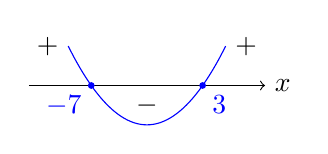
\begin{tikzpicture}
            \def\a{0.5}
            \draw[->] (-1.5,0) -- (1.5,0) node[right] {$x$};
            \draw[domain=-1:1,smooth,variable=\x,blue] plot ({\x},{(\x)^2 - \a});
            \filldraw[blue] ({-sqrt(\a)},0) circle (1pt) node[below left] {$-7$};
            \filldraw[blue] ({sqrt(\a)},0) circle (1pt) node[below right] {$3$};
            \node[right] at (1,0.5) {$+$};
            \node[left] at (-1,0.5) {$+$};
            \node[above] at (0,-0.5) {$-$};
          \end{tikzpicture}
        \end{note}
        $x<-7$ and $x>3$
      }
      \task $ 2x^2 + x < 3 $;
      {
        \begin{note}
          $2x^2 + x -3 < 0$

          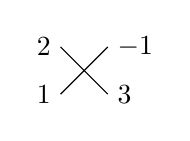
\begin{tikzpicture}
            \def\a{0.3}
            \draw[-] (-\a,\a) node[left] {$2$} -- (\a,-\a) node[right] {$3$};
            \draw[-] (-\a,-\a) node[left] {$1$} -- (\a,\a) node[right] {$-1$};
          \end{tikzpicture}

          $ (2x+3)(x-1) < 0 $

          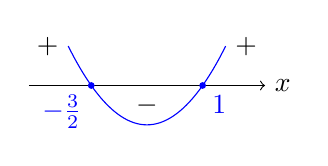
\begin{tikzpicture}
            \def\a{0.5}
            \draw[->] (-1.5,0) -- (1.5,0) node[right] {$x$};
            \draw[domain=-1:1,smooth,variable=\x,blue] plot ({\x},{(\x)^2 - \a});
            \filldraw[blue] ({-sqrt(\a)},0) circle (1pt) node[below left] {$-\frac{3}{2}$};
            \filldraw[blue] ({sqrt(\a)},0) circle (1pt) node[below right] {$1$};
            \node[right] at (1,0.5) {$+$};
            \node[left] at (-1,0.5) {$+$};
            \node[above] at (0,-0.5) {$-$};
          \end{tikzpicture}
        \end{note}
        $-\frac{3}{2} < x < 1$
      }
      \task $ 4x^2 + 10x - 6 < 0 $;
      {
        \begin{note}
          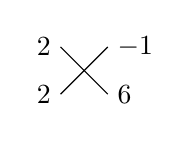
\begin{tikzpicture}
            \def\a{0.3}
            \draw[-] (-\a,\a) node[left] {$2$} -- (\a,-\a) node[right] {$6$};
            \draw[-] (-\a,-\a) node[left] {$2$} -- (\a,\a) node[right] {$-1$};
          \end{tikzpicture}

          $ (2x+6)(2x-1) < 0 $

          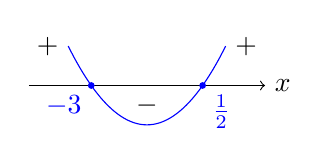
\begin{tikzpicture}
            \def\a{0.5}
            \draw[->] (-1.5,0) -- (1.5,0) node[right] {$x$};
            \draw[domain=-1:1,smooth,variable=\x,blue] plot ({\x},{(\x)^2 - \a});
            \filldraw[blue] ({-sqrt(\a)},0) circle (1pt) node[below left] {$-3$};
            \filldraw[blue] ({sqrt(\a)},0) circle (1pt) node[below right] {$\frac{1}{2}$};
            \node[right] at (1,0.5) {$+$};
            \node[left] at (-1,0.5) {$+$};
            \node[above] at (0,-0.5) {$-$};
          \end{tikzpicture}
        \end{note}
        $-3<x<\frac{1}{2}$
      }
      \task $ x^2 + 2x + 4 > 0 $;
      {
        \begin{note}
          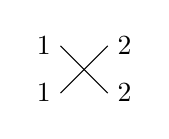
\begin{tikzpicture}
            \def\a{0.3}
            \draw[-] (-\a,\a) node[left] {$1$} -- (\a,-\a) node[right] {$2$};
            \draw[-] (-\a,-\a) node[left] {$1$} -- (\a,\a) node[right] {$2$};
          \end{tikzpicture}

          $ (x+2)^2 > 0 $

          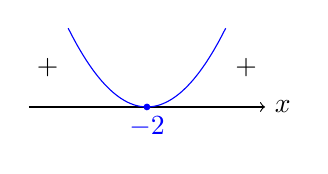
\begin{tikzpicture}
            \def\a{0.5}
            \draw[->] (-1.5,0) -- (1.5,0) node[right] {$x$};
            \draw[domain=-1:1,smooth,variable=\x,blue] plot ({\x},{(\x)^2});
            \filldraw[blue] (0,0) circle (1pt) node[below] {$-2$};
            \node[right] at (1,0.5) {$+$};
            \node[left] at (-1,0.5) {$+$};
          \end{tikzpicture}
        \end{note}
        all x
      }
    \end{tasks}
  \end{solution}
  \item Recall that $\sqrt{a}$ is a real number if and only if $a \geq 0$, and find the values of $x$ for which each of the following is a real number:
  \begin{tasks}(2)
    \task $\sqrt{4-x^2}$;
    \task $\sqrt{x^2-9}$;
    \task \(\frac{1}{\sqrt{4-3x}}\);
    \task \(\frac{1}{\sqrt{x^2-x-12}}\);
  \end{tasks}
  \item Find the values of $x$ for which each of the following is positive:
  \begin{tasks}(2)
    \task \(\frac{x}{x^2+4}\);
    \task \(\frac{x}{x^2-4}\);
    \task \(\frac{x+1}{x-3}\);
    \task \(\frac{x^2-1}{x^2-3x}\);
  \end{tasks}
  \item State the values of $a$ for which the following inequalities are valid:
  \begin{tasks}(2)
    \task $a \leq a$;
    \task $a<a$;
  \end{tasks}
  \item If $a \leq b$ and $b \leq a$, what conclusion can be drawn about $a$ and $b$?
  \item \begin{tasks}
    \task If $a<b$ is true, is it also necessarily true that $a \leq b$?
    \task If $a \leq b$ is true, is it also necessarily true that $a<b$?
  \end{tasks}
  \item State whether each pair of points lies on a horizontal or a vertical line:
  \begin{tasks}(2)
    \task $(-2, -5)$, $(-2, -3)$;
    \task $(-2, -5)$, $(7, -5)$;
    \task $(-3, 4)$, $(6, 4)$;
    \task $(2, -11)$, $(2, 5)$;
    \task $(2, 2)$, $(-13, 2)$;
    \task $(-7, -7)$, $(-7, 7)$;
    \task $(3, 5)$, $(3, -2)$;
    \task $(-1, -2)$, $(2, -2)$.
  \end{tasks}
  \item Three vertices of a rectangle are $(-1, 2)$, $(3, -5)$, $(-1, -5)$. What is the fourth vertex?
\end{questions}